\documentclass{standalone}
\usepackage{tikz}
\usepackage{ctex,siunitx}
\setCJKmainfont{Noto Serif CJK SC}
\usepackage{tkz-euclide}
\usepackage{amsmath}
\usepackage{wasysym}
\usetikzlibrary{patterns, calc}
\usetikzlibrary {decorations.pathmorphing, decorations.pathreplacing, decorations.shapes,}
\begin{document}
\small
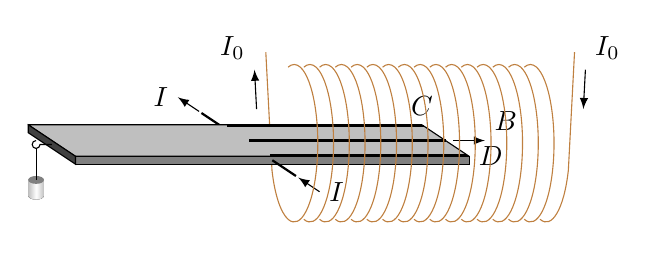
\begin{tikzpicture}[>=latex,scale=1.0]
  \draw[brown](0.5,-1.0)arc(-105:-160: 0.3 and 1)--++(93:1.5);
  \draw[thin,->](0.1,0.4)--++(93:0.5)node[above left]{$I_0$};
  \draw[->](2.6,0)--(3.0,0)node[above right]{$B$};
  \draw[thick](-0.3,0.15)--++(-0.3,0.2);
  \draw[fill=lightgray,line join=round](-2.8,0.2)--(2.2,0.2)node[above]{$C$}--(2.8,-0.2)node[right]{$D$}--(-2.2,-0.2)--cycle;
  \draw[fill=gray](2.8,-0.2)rectangle(-2.2,-0.3);
  \draw[fill=darkgray](-2.8,0.2)--(-2.2,-0.2)--(-2.2,-0.3)--(-2.8,0.1)--cycle;
  \draw[thick](2.5,0)--(0,0)(-0.27,0.18)--++(2.5,0)(0.27,-0.18)--++(2.5,0);
  \draw[thick](0.3,-0.25)--++(0.3,-0.2);
  \draw[->](0.9,-0.65)--++(-0.27,0.18)node[at start,right]{$I$};
  \draw[<-](-0.9,0.55)--++(0.27,-0.18)node[at start,left]{$I$};
  \draw[thin](-2.5,-0.05)--(-2.65,-0.05)arc(360:90:0.05);
  \fill[left color=lightgray,right color=lightgray,middle color=white](-2.7,-0.7)ellipse(0.1 and 0.05);
  \fill[left color=lightgray,right color=lightgray,middle color=white](-2.8,-0.7)rectangle(-2.6,-0.5);
  \fill[gray](-2.7,-0.5)ellipse(0.1 and 0.05);
  \draw(-2.7,-0.1)--(-2.7,-0.5);
  \foreach \x in {0.5,0.7,...,3.6}
  {
    \draw[brown](\x,-1.0)arc(-105:105: 0.3 and 1);
  }
  \draw[brown](3.7,-1.0)arc(-105:-20: 0.3 and 1)--++(87:1.5);
  \draw[thin,<-](4.25,0.4)--++(87:0.5)node[above right]{$I_0$};
\end{tikzpicture}
\end{document}